\documentclass[11pt]{article}

\marginparwidth 0.5in 
\oddsidemargin 0.25in 
\evensidemargin 0.25in 
\marginparsep 0.25in
\topmargin 0.25in 
\textwidth 6in
\textheight 8 in

\usepackage{graphicx}
\usepackage{float}

\begin{document}
\author{Zhong-Xi Lu \& Thomas Van Bogaert}
\title{\textbf{Distributed Systems} \\ \Large{Chat Manual}}
\date{}
\maketitle

\section{Used Technologies}

\begin{itemize}
	\item Java EE
	\item HTML, CSS (Bootstrap), JS, AJAX
	\item Servlets, Beans, Entity Classes
	\item GlassFish Server
	\item JavaDB
	\item socat
	\item Netbeans
\end{itemize}

\section{Set up}

\subsection{Set up database server}
\begin{enumerate}
	\item Open Netbeans
	\item Open the Services tab
	\item Expand 'Databases'
	\item Right click 'Java DB' and select 'Create Database...'
	\begin{figure}[H]
		\centering
		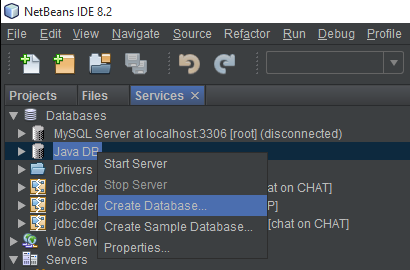
\includegraphics[height=50mm]{select_create_db.png}
	\end{figure}
	\item Enter the following:
	\begin{figure}[H]
		\centering
		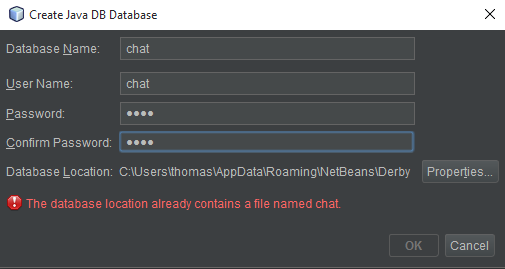
\includegraphics[height=50mm]{select_create_db2.png}
	\end{figure}
	With the password being "chat" and click 'OK'

	\item Open a terminal and cd to \texttt{'groep\_8/socat'}
	\item Set execute permissions on \texttt{socat/build\_socat} (\texttt{chmod +x build\_socat.sh})
	\item Run \texttt{./build\_socat.sh} (socat will run after it is compiled. socat needs to be running to access the database from a remote server.)
\end{enumerate}

\subsection{Set up client servers}
\subsubsection{For each server}
\begin{enumerate}
	\item Open Netbeans
	\item Open the Chat project by selecting 'File' $\rightarrow$ 'Open Project...'
	\begin{figure}[H]
		\centering
		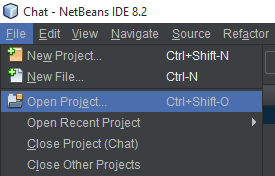
\includegraphics[height=40mm]{open_project.png}
	\end{figure}
	then find the location of the Chat project (\texttt{groep\_8/Chat})
	\item Open the Services tab
	\item Right click 'Databases' and select 'New Connection...'
	\item Select the 'Java DB (Network)' driver and click 'Next'
	\begin{figure}[H]
		\centering
		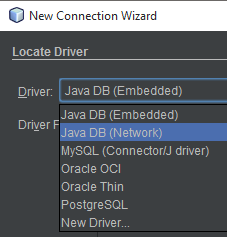
\includegraphics[height=45mm]{select_db_driver.png}
	\end{figure}
	\item Enter the following:
	\begin{figure}[H]
		\centering
		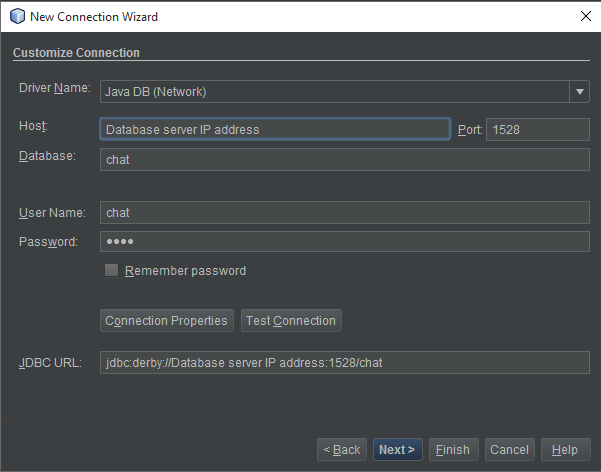
\includegraphics[height=50mm]{new_db_connection.png}
	\end{figure}
	With 'Database server IP address' the IP address of the server on which the database is running and as Password 'chat'. Then click 'Finish'
	

	
	\item Open the Projects tab
	\item Expand 'Chat'
	\item Expand 'Configuration Files'
	\item Open \texttt{glassfish-resources.xml}
	\item Enter the IP address of the database server in the following locations in \texttt{glassfish-resources.xml}:
	\begin{figure}[H]
		\centering
		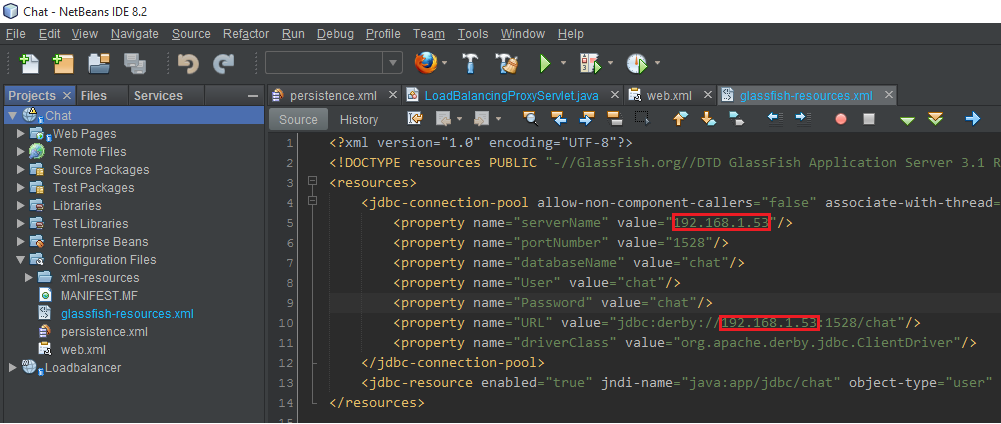
\includegraphics[height=70mm]{enter_db_ip_gf_resources.png}
	\end{figure}
	\item Right click on the 'Chat' project and click 'Deploy'
\end{enumerate}
\subsubsection{On only one client server}
\begin{enumerate}
	\item Open the \texttt{create\_tables.sql} file by selecting 'File' $\rightarrow$ 'Open Project...'
	\begin{figure}[H]
		\centering
		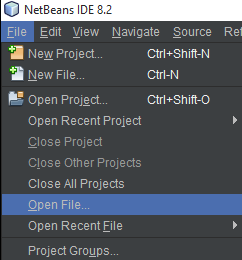
\includegraphics[height=40mm]{open_file.png}
	\end{figure}
	then open the location of the \texttt{create\_tables.sql} file (\texttt{groep\_8/db/create\_tables.sql})
	\item Right click in the file and select 'Run File'.
	\item Select the newly created database connection and click 'OK'.
\end{enumerate}

\subsection{Set up load balancer}
\begin{enumerate}
	\item Copy the maven repository to the right location:
	\begin{enumerate}
		\item \texttt{$\sim$: mkdir .m2}
		\item \texttt{$\sim$: cp -a groep\_8/maven\_repo/. $\sim$/.m2 }
	\end{enumerate}
	\item Open the Loadbalancer project in Netbeans
	\item Open the Projects tab
	\item Expand 'Loadbalancer' $\rightarrow$ 'Source Packages' $\rightarrow$ 'Servlets'
	\item Open the 'LoadBalancingProxyServlet.java' file
	\item Change the IP addresses in the 'LoadBalancingProxyServlet.java' file to the IP addresses of the servers running the Chat application
	\begin{figure}[H]
		\centering
		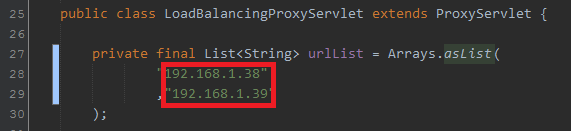
\includegraphics[height=30mm]{set_server_ip_addresses.png}
	\end{figure}
	\item Deploy the Loadbalancer the same way as we did the Chat applications.
\end{enumerate}
If everything went right, the load balanced Chat application is accessible at \texttt{\{IP address of load balancer server\}:8080/Loadbalancer}
\section{Architecture}

\begin{figure}[H]
\centering
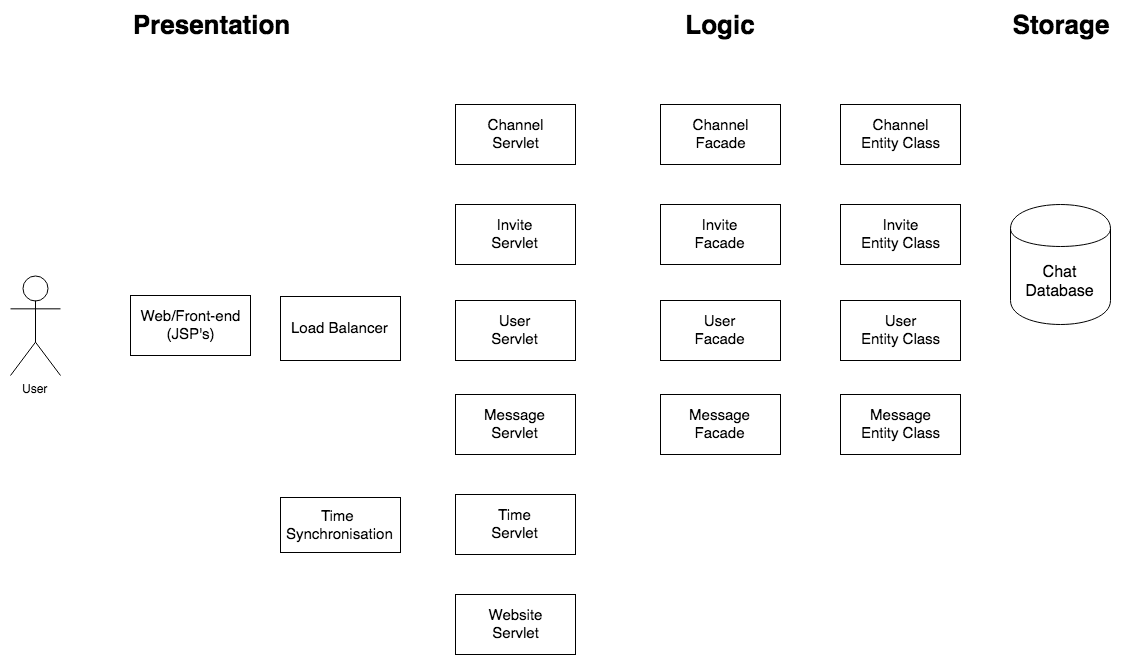
\includegraphics[height=100mm]{architecture.png}
\caption{Chat Login Page}
\end{figure}

This is our service oriented architecture. In the front-end, we have jsp's that makes requests to the server through the load balancer. The load balancer forwards this request to the appropiate server/servlet. Each servlet then makes calls to the facades that is responsible for all the business logic. If a change to the database needs to be done, a facade can rely on an interface of the database (entity classes).

\section{Design Choices}

As previously mentioned, we tried to make a layered architecture (service-oriented). This way, each layer has one responsibility; servlets are responsible for handling requests, facades for doing all the logic, entity classes for the communication with the database. On the front-end, we have jsp's that can easily process all the data received from the server. Furthermore, we make ajax calls to the server, because it's reasonably fast and you can easily manipulate the responses and integrate it in your jsp's. Above that, those call are asynchronous, which makes it a lot easier to send different requests at roughly the same time.

\section{Chat Tutorial}

\begin{figure}[H]
\centering
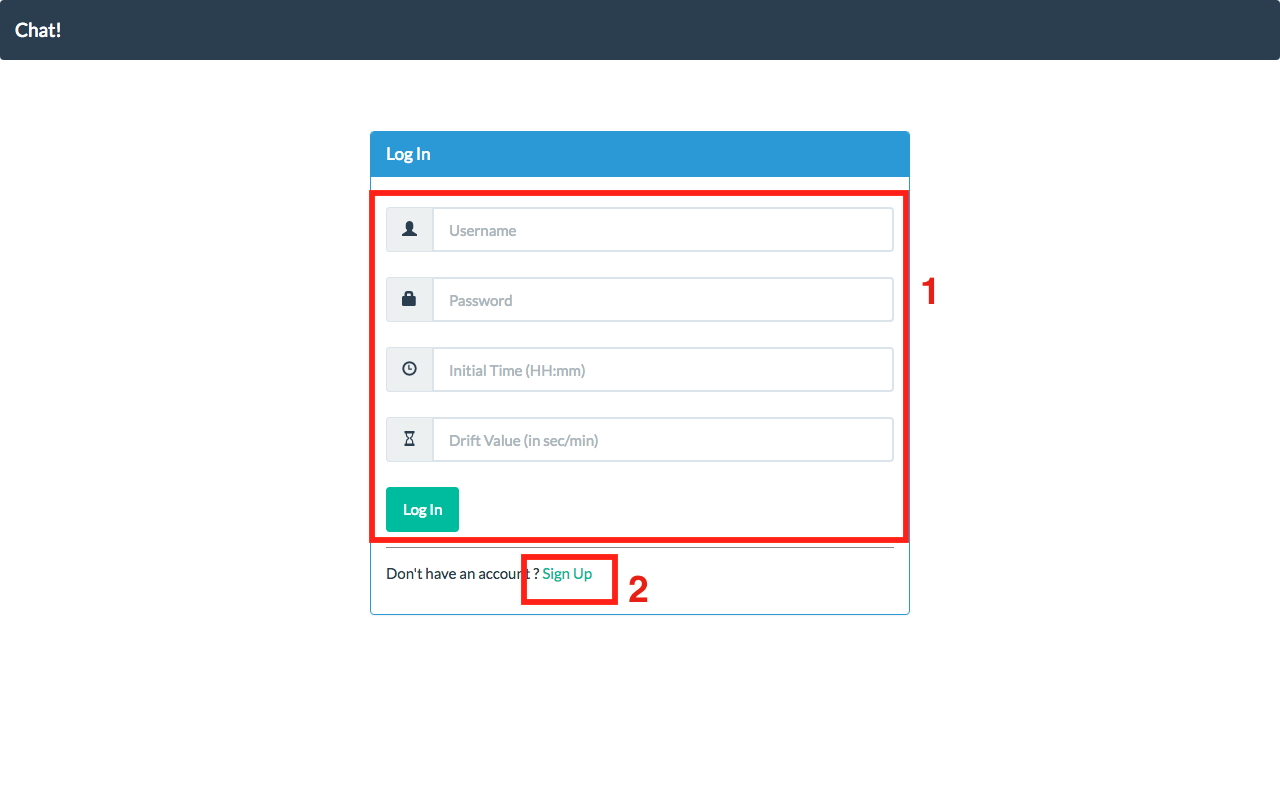
\includegraphics[height=100mm]{login.png}
\caption{Chat Login Page}
\end{figure}

If a user browses to our chat application the page above will be shown.

\begin{enumerate}
	\item A user can login by filling in the necessary information. Note that an initial time (HH:mm) and drift value must be specified.
	\item Or, if the user doesn't have an account yet, he/she can create one here.
\end{enumerate}

\begin{figure}[H]
\centering
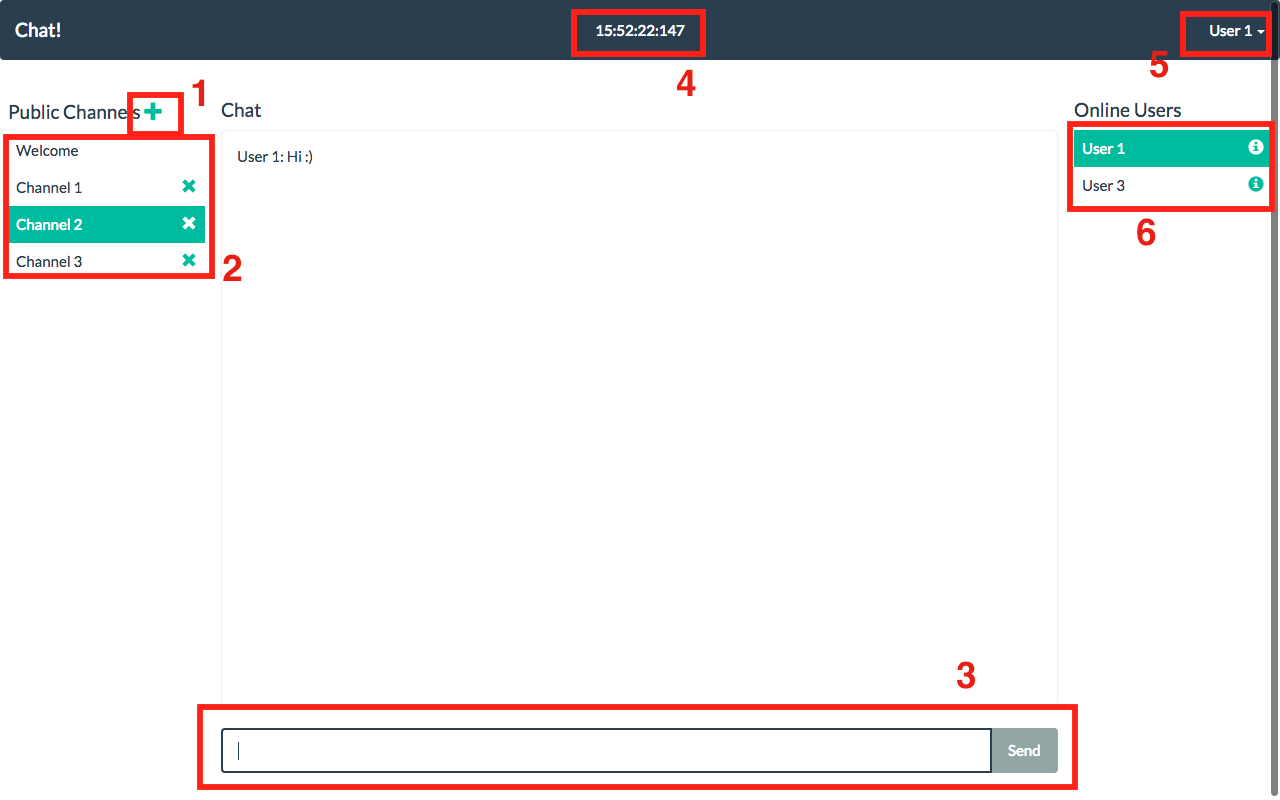
\includegraphics[height=100mm]{chat.png}
\caption{Chat Homepage}
\end{figure}

The figure above shows the main screen when the user has logged in or registered. The user can do the following:

\begin{enumerate}
	\item If the user is a moderator, a new public channel can be added by clicking the plus-sign. After this, a window will pop up where a name for the channel must be specified.
	\item Here, a list of all the active public channel are shown (green indicates the channel of the user); the user can simply join a channel by clicking on it. If the user is a moderator, the channel can be removed as well by clicking the X-sign next to the channel name.
	\item This is the input field to send a message to the current channel of the user. The message will then appear in the chat box displayed above.
	\item The current time for this specific user is shown here and is synchronised every 10 seconds with the server.
	\item A user can log out by clicking on his username and selecting the "Log out" option.
	\item All the current online users are shown here (green indicates the name of the user and red indicates a moderator). By clicking on a user, you can invite them to a private channel (a channel name must be given as well), the other user can then accept or decline the invite. In addition, a moderator can also view all the messages a user sent (in all public/private channels) by clicking the info-sign next to the name. This will one a new page with the history of that user.
\end{enumerate}


\end{document}
